% sage_latex_guidelines.tex V1.20, 14 January 2017

\documentclass[Afour,sageh,times]{sagej}

\usepackage{moreverb,url}

\usepackage[colorlinks,bookmarksopen,bookmarksnumbered,citecolor=red,urlcolor=red]{hyperref}
\usepackage{setspace}
\usepackage{tabularx}
\usepackage{booktabs}
\usepackage{booktabs}
\usepackage{array}
\usepackage{longtable}
\usepackage{amsmath}
\usepackage{xcolor}
\usepackage{colortbl}
\usepackage{caption}

\definecolor{headerblue}{RGB}{44, 62, 80}
\definecolor{rowgray}{RGB}{245, 245, 245}
\definecolor{sectiongreen}{RGB}{39, 174, 96}


\newcommand\BibTeX{{\rmfamily B\kern-.05em \textsc{i\kern-.025em b}\kern-.08em
T\kern-.1667em\lower.7ex\hbox{E}\kern-.125emX}}

\def\volumeyear{2026}

\begin{document}
\setstretch{1.5} 
\runninghead{Caterer}

\title{A Bistable Ordinary Differential Equations Model of Mechanotransduction in Cardiac Fibrosis}

\author{Zachary Caterer\affilnum{1,2}}

\affiliation{\affilnum{1}Department of Chemical and Biological Engineering, University of Colorado Boulder, Boulder CO, USA\\
\affilnum{2}Department of Biomedical Informatics, University of Colorado Anschutz, Aurora, CO, USA}


\begin{abstract}

Myocardial infarction often leads to fibrotic remodeling of the heart, which can impair ventricular function. After injury, fibroblasts differentiate into myofibroblasts and produce collagen to repair the damaged tissue. Because myofibroblasts are mechanosensitive, increased matrix stiffness can promote further activation and collagen production, creating a positive feedback loop that sometimes lead to persistent fibrosis. In this project, we construct a simple system of ordinary differential equations describing fibroblasts ($F$), myofibroblasts ($M$), collagen ($C$), and matrix metalloproteinases ($M$). Matrix stiffness is modeled as a function of collagen accumulation, and fibroblast activation is represented using a Hill-type inflammatory and stiffness response. Numerical simulations were performed in Python to evaluate the behavior of the system. The model shows bistable dynamics with a low-stiffness healthy state and a high-stiffness fibrotic state resulting from inflammatory status. Simulations also indicate that small or short inflammatory signals resolve without permanent fibrosis, while sufficiently strong perturbations push the system into a persistent fibrotic state. These results suggest that mechanosensitive feedback can produce a threshold beyond which fibrosis becomes self-sustaining.

\end{abstract}


\keywords{Matrix Metalloproteinases, Matrix Stiffness, Myocardial Infarction,
Myofibroblasts, Ordinary Differential Equations, Modeling Method
}

\maketitle

\section{Introduction}
\label{sec:intro}
Myocardial infarction (MI) remains a leading cause of congestive heart failure, affecting hundreds of thousands of patients annually~\citep{mozaffarian2016heart,hellermann2005heart,anavekar2004relation}. Following infarction, the left ventricle undergoes a complex remodeling process in which necrotic myocytes are replaced by fibrotic scar tissue, primarily mediated by cardiac fibroblasts and their activated counterparts, myofibroblasts~\citep{cohn2000cardiac, segers2008stem}. In normal wound healing, this fibrotic response is transient and self-limiting. However, in pathological fibrosis, myofibroblast activation persists, collagen accumulates excessively, and the myocardium stiffens irreversibly, subsequently affecting diastolic filling, disrupting the propagation of action potentials, and driving progressive heart failure~\citep{song2012heart, hinz2007formation, spinale2007myocardial, gaudron2001time, pfeffer1991progressive}.

Myofibroblasts are sensitive to the mechanical properties of their surrounding extracellular matrix (ECM)~\citep{hinz2010myofibroblast}. As myofibroblasts deposit collagen, increasing the matrix stiffness, which in turn promotes further differentiation from fibroblast-to-myofibroblast, creating a positive feedback loop~\citep{younesi2024fibroblast, gibb2020myofibroblasts}. Transforming growth factor-$\beta$ (TGF-$\beta$), a cytokine secreted by macrophages and fibroblasts in response to injury, acts synergistically with mechanical stiffness to amplify this response~\citep{tiskratok2025extracellular, frangogiannis2022transforming, frangogiannis2020transforming}. The result is a system with hallmarks of bistability: at low inflammatory stimulus, the system resolves back to homeostasis, and above some critical inflammatory threshold, fibrosis is irreversible.

Prior computational work has made important progress in modeling cardiac remodeling as a system of coupled ordinary differential equations (ODEs). Jin et al. (2011)~\citep{jin2011combining} established a foundational ODE framework tracking macrophage density, fibroblast density, TGF-$\beta$, matrix metalloproteinase (MMP-9), and collagen concentration post-MI, demonstrating that the balance between ECM synthesis and degradation governs remodeling outcomes. More recently, Chowkwale et al. (2023)~\citep{chowkwale2023} extended this approach to an intercellular model incorporating neutrophils, monocytes, macrophages, fibroblasts, and multiple cytokines (IL-1$\beta$, Tumor Necrosis Factor (TNF)-$\alpha$, granulocyte macrophage-colony stimulating factor (GM-CSF), TGF-$\beta$, MMP-9), predicting that post-MI inflammation is a graded response to infarct size while collagen deposition behaves as an ultrasensitive switch, exhibiting a Hill coefficient of 9.56 with respect to infarct size. On the biological side, Kim et al. (2018)~\citep{kim2018} reviewed the mechanobiological mechanisms underlying myofibroblast fate, highlighting the roles of substrate stiffness, cyclic strain, ECM directionality, and key signaling pathways including RhoA/ROCK~\citep{jenkins2006ligation, wipff2007myofibroblast}, YAP/TAZ~\citep{liu2015mechanosignaling, mosqueira2014hippo, yang2014mechanical}, p38 MAPK~\citep{molkentin2017fibroblast, wang2000force}, and MRTF~\citep{huang2012matrix} in driving transdifferentiation. Despite this body of work, a minimal ODE model that explicitly couples mechanical stiffness to fibroblast activation, and characterizes the bistable switch that separates reversible from irreversible fibrosis, has not been developed.

Here, we develop a minimal ODEs model of mechanotransduction in cardiac fibrosis, tracking fibroblast and myofibroblast populations, collagen concentration, MMP-9 levels, and matrix stiffness. The model captures the key positive feedback between collagen deposition and stiffness-driven myofibroblast activation, along with the regulatory role of MMP-9-mediated collagen degradation. Using this framework, we identify parameter combinations that control the bistability threshold and show that the system exhibits two distinct outcomes, (1) resolution of healing when inflammation is low, and (2) commitment to fibrosis when inflammation exceeds a critical threshold. We further examine the system’s response to repeated low- and high-amplitude inflammatory pulses to test whether transient perturbations can push the system into the fibrotic state. Finally, a sensitivity analysis of the key parameters evaluates how robust this threshold behavior is to parameter variation and highlights processes that most strongly influence fibrotic outcomes.


\section{Methods}

\subsection{Model Overview}

To investigate mechanotransduction-driven fibrosis following myocardial infarction, we developed a reduced-order computational model describing the coupled dynamics of fibroblast activation, extracellular matrix deposition, and matrix degradation. The model is based on regulatory interactions described in previously published computational models of post-infarction inflammation and fibrosis by Chowkwale et al.\ \cite{chowkwale2023}, but simplified to focus on the minimal mechanotransduction feedbacks capable of producing bistable fibrotic outcomes.

\begin{figure}
    \centering
    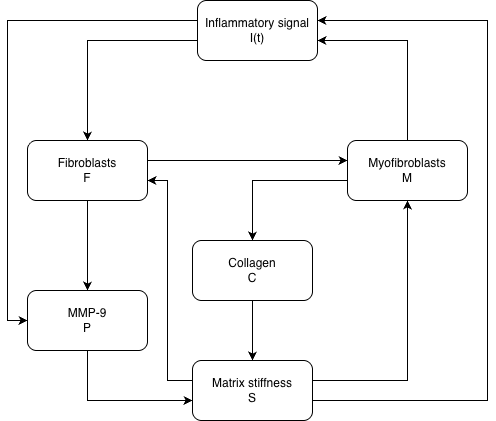
\includegraphics[width=0.5\textwidth]{figures/drawio.png}
    \caption{Conceptual causal diagram of the mechanotransduction model. Arrows indicate directional regulatory interactions between model components. Complete model not represented, and model in figure not fully represented in this work.}
    \label{fig:model_schem}
\end{figure}

The model consists of four coupled ODEs describing the evolution of key cellular and extracellular components of the fibrotic microenvironment. State variables are summarized in Table \ref{tab:variables}, and model parameters are listed in Table \ref{tab:parameters}. The directed acyclical graph of the model is illustrated in Figure~\ref{fig:model_schem}.

\begin{table*}[h]
\centering
\begin{tabularx}{\textwidth}{lXX}
\toprule
\textbf{Variable} & \textbf{Description} & \textbf{Units}\\
\midrule
$F$ & Fibroblast density & cells mm$^{-3}$ \\
$M$ & Myofibroblast density & cells mm$^{-3}$ \\
$C$ & Collagen concentration & mg mm$^{-3}$ \\
$P$ & Matrix metalloproteinase-9 (MMP-9) concentration & nM \\
\bottomrule
\end{tabularx}
\caption{State variables in the fibrosis model.}
\label{tab:variables}
\end{table*}

It is important to note that matrix stiffness $S$ and inflammatory signal $I$ are not state variables integrated by the ODE system; rather, they are computed algebraically from the state variables and time at each integration step, as described below.

\begin{table*}[h]
\centering
\begin{tabularx}{\textwidth}{lXlX}
\toprule
\textbf{Parameter} & \textbf{Description} & \textbf{Value} & \textbf{Units}\\
\midrule
$\lambda_I$ & Inflammation-driven fibroblast recruitment rate & 1.2 & day$^{-1}$ \\
$\lambda_S$ & Stiffness-driven fibroblast recruitment rate & 1.0 & day$^{-1}$ \\
$F_\mathrm{max}$ & Fibroblast crowding limit & 1.0 & cells mm$^{-3}$ \\
$\delta_F$ & Fibroblast death rate & 0.25 & day$^{-1}$ \\
$k_{FM}$ & Fibroblast-to-myofibroblast conversion rate & 0.4 & day$^{-1}$ \\
$\beta$ & Stiffness feedback amplification exponent & 1.7 & dimensionless \\
$\delta_M$ & Myofibroblast decay rate & 0.3 & day$^{-1}$ \\
$k_C$ & Collagen production rate by myofibroblasts & 0.6 & mg mm$^{-3}$ day$^{-1}$ \\
$\delta_C$ & Collagen degradation rate & 0.02 & day$^{-1}$ \\
$k_s$ & Collagen-to-stiffness scaling coefficient & 1.5 & kPa (mg mm$^{-3}$)$^{-1}$ \\
$S_0$ & Baseline matrix stiffness & 0.05 & kPa \\
$k_{P,F}$ & MMP-9 production rate by fibroblasts & 0.3 & nM mm$^{3}$ cell$^{-1}$ day$^{-1}$ \\
$k_{P,I}$ & Inflammation-driven MMP-9 production rate & 0.6 & nM day$^{-1}$ \\
$\delta_P$ & MMP-9 degradation rate & 0.4 & day$^{-1}$ \\
\bottomrule
\end{tabularx}
\caption{Model parameters governing fibrosis dynamics.}
\label{tab:parameters}
\end{table*}

\subsection{Inflammatory Signal}
The inflammatory signal $I(t)$ is not a state variable but rather an externally prescribed time-varying input representing the aggregate cytokine-driven immune activity following MI. Rather than explicitly modeling each signaling pathway, this term captures the combined effect of macrophage signaling and key pro-inflammatory mediators (e.g., including macrophages, IL-1$\beta$ TNF-$\alpha$, granulocyte-macrophage colony-stimulating factor (GM-CSF), etc) described in the model of Chowkwale et al.~\citep{chowkwale2023}. The goal of this formulation is to provide a simplified representation of the inflammatory phase of post-infarction healing sufficient to drive fibroblast recruitment and MMP-9 production, without reproducing the full cytokine network.

Three inflammatory signal forms were used across the simulation scenarios. The baseline healthy signal decays exponentially following the initial infarction event:

\begin{equation}\label{eq:inflam-healthy}
I(t) = e^{-0.4\cdot t}
\end{equation}

To simulate repeated secondary inflammatory insults, Gaussian pulses are superimposed on the baseline signal:

\begin{equation}\label{eq:inflam-pulse}
I(t) = e^{-0.4\cdot t} + \sum_{j} A \exp\!\left(-\frac{(t - t_j)^2}{2\cdot w^2}\right)
\end{equation}

where $t_j$ are the pulse center times, $A$ is the pulse amplitude, and $w$ is the pulse width. Two pulse regimes consist of sub-threshold pulses ($A=0.1$, $w=0.5$) and supra-threshold pulses ($A=0.4$, $w=0.7$), both applied at $t=5,10,15,20,25$ days post-MI.

For the chronic inflammation scenario, a two-component exponential signal is used in place of Equation~\ref{eq:inflam-pulse}:

\begin{equation}\label{eq:chron-inflam}
I(t) = e^{-0.4\cdot t} + 0.12 \cdot e^{-0.02\cdot t}
\end{equation}

The second term represents a slowly decaying persistent immune component, mimicking prolonged low-level cytokine secretion associated with cardiometabolic comorbidities or repeated subclinical ischaemic events. The decay rate of 
$0.02\sim$day$^{-1}$ corresponds to a half-life of approximately 35~days, ensuring that the chronic signal remains biologically active across the full 30-day simulation window.


\subsection{Matrix Stiffness}

Matrix stiffness $S$ is computed as a nonlinear function of collagen concentration~\citep{gachon2020stretching}, capturing the well-documented superlinear relationship between collagen content and tissue mechanical properties:

\begin{equation}\label{eq:stiffness}
S = S_0 + k_s\, C^{\,\beta}
\end{equation}

where $S_0$ is the baseline stiffness of healthy myocardium, $k_s$ is a scaling coefficient, $C$ is the collagen concentration, and $\beta > 1$ is an amplification exponent that captures the nonlinear stiffening behavior observed as collagen accumulates. 

\subsection{Fibroblast Dynamics}

Fibroblast density evolves through a combination of recruitment driven by both inflammatory signals and matrix stiffness, logistic crowding, constitutive turnover, and conversion to the myofibroblast phenotype:

\begin{equation}
\begin{aligned}
\frac{dF}{dt} = &
\left(\lambda_I I + \lambda_S S\right) F 
\left(1 - \frac{F}{F_\mathrm{max}}\right) \\
&- (\delta_F + k_{FM})F
\end{aligned}
\end{equation}

The logistic term $(1 - F/F_\mathrm{max})$ limits unbounded fibroblast expansion by imposing a crowding effect analogous to that described in Jin et al.~\citep{jin2011combining} and Chowkwale et al.~\citep{chowkwale2023}. The conversion term $k_{FM} F$ represents constitutive fibroblast-to-myofibroblast activation, which is indirectly stiffness-dependent since elevated $S$ feeds back to increase fibroblast recruitment.

\subsection{Myofibroblast Dynamics}

Myofibroblasts arise from fibroblast activation and are additionally amplified by a stiffness-dependent self-reinforcing term:

\begin{equation}\label{eq:myofibroblasts}
\frac{dM}{dt} = k_{FM}\, F + \beta\, S\, M - \delta_M\, M
\end{equation}

The term $\beta S M$ captures the mechanotransduction positive feedback loop such that elevated matrix stiffness promotes further myofibroblast activation and survival. Myofibroblasts are lost through apoptosis or phenotypic reversion at rate $\delta_M$.

\subsection{Collagen Dynamics}

Extracellular matrix accumulation is driven by the rate of myofibroblast collagen synthesis ($k_C$) and opposed by the rate of collagen degradation ($\delta_C$):

\begin{equation}\label{eq:collagen}
\frac{dC}{dt} = k_C\, M - \delta_C\, C
\end{equation}

\subsection{MMP-9 Dynamics} \label{sec:mmp9}

Matrix metalloproteinase-9 is produced by both fibroblasts ($k_{P,F}$) and in response  to the inflammatory signal ($k_{P,I}$. It undergoes natural degradation ($\delta_P$) and is consumed through collagen-binding and cleavage reactions ($k_{PC}$):

\begin{equation}
\frac{dP}{dt} = k_{P,F}\, F + k_{P,I}\, I - \delta_P\, P - k_{PC}\, P\, C
\end{equation}

\subsection{Numerical Implementation}

The system of four coupled ODEs was integrated using \texttt{scipy.integrate.odeint} in Python, which implements the LSODA algorithm with adaptive step-size control. All simulations were run from $t = 0$ to $t = 30$ days on a uniform grid of 1000 time points. Initial conditions were set to $F_0 = 0.01$ cells mm$^{-3}$, $M_0 = 0$ cells mm$^{-3}$, $C_0 = 0.01$ mg mm$^{-3}$, and $P_0 = 0$ nM, representing a sparse post-infarction cellular environment with minimal initial matrix density.

Four simulation scenarios were evaluated: (1) baseline healthy healing with only the exponentially decaying MI signal (eq~\ref{eq:inflam-healthy}); (2) chronic inflammation modeled using equation~\ref{eq:chron-inflam} representing prolonged low-level immune activation; (3) small repeated pulses at five discrete time points ($t = 5, 10, 15, 20, 25$ days; $A = 0.1$, $w = 0.5$, using equation~\ref{eq:inflam-pulse}); and (4) large repeated pulses at the same five time points ($A = 0.4$, $w = 0.7$, using equation~\ref{eq:inflam-pulse}).

\subsection{Sensitivity Analysis}

To identify which model parameters most strongly govern steady-state fibrosis, a local sensitivity analysis was performed using finite differences. For each parameter $k_i$, a normalized sensitivity coefficient was computed as:

\begin{equation} \label{eq:sensitivity}
\begin{aligned}
    S_i &
    = \frac{\partial Y}{\partial k_i}\frac{k_i}{Y} \\
    & \approx \frac{Y(k_i + \Delta k_i/2) - Y(k_i - \Delta k_i/2)}{\Delta k_i \cdot Y(k_i)} \cdot k_i
\end{aligned}
\end{equation}

where $Y$ is the steady-state collagen concentration $C(t = 30)$ and $\Delta k_i = 0.1\, k_i$ (i.e., a 10\% symmetric perturbation). The following twelve parameters were evaluated: $\lambda_I$, $\lambda_S$, $\delta_F$, $k_{FM}$, $\beta$, $\delta_M$, $k_C$, $\delta_C$, $k_s$, $k_{P,F}$, $k_{P,I}$, and $\delta_P$. Parameters with sensitivity coefficients indistinguishable from zero were excluded from the final figure. 

\section{Results and Discussion}
\label{sec:results}

All simulations were run for a 30-day post-infarction window using the ODE system described in the Methods Section. All model outputs were min-max normalized to $[0, 1]$ within each simulation so the time evolution of different variables could be compared visually, consistent with the work in Chowkwale et al. \citep{chowkwale2023}.

\subsection{Healthy Healing and Chronic Fibrosis}
\label{subsec:healthy-chronic}

\begin{figure*}
    \centering
    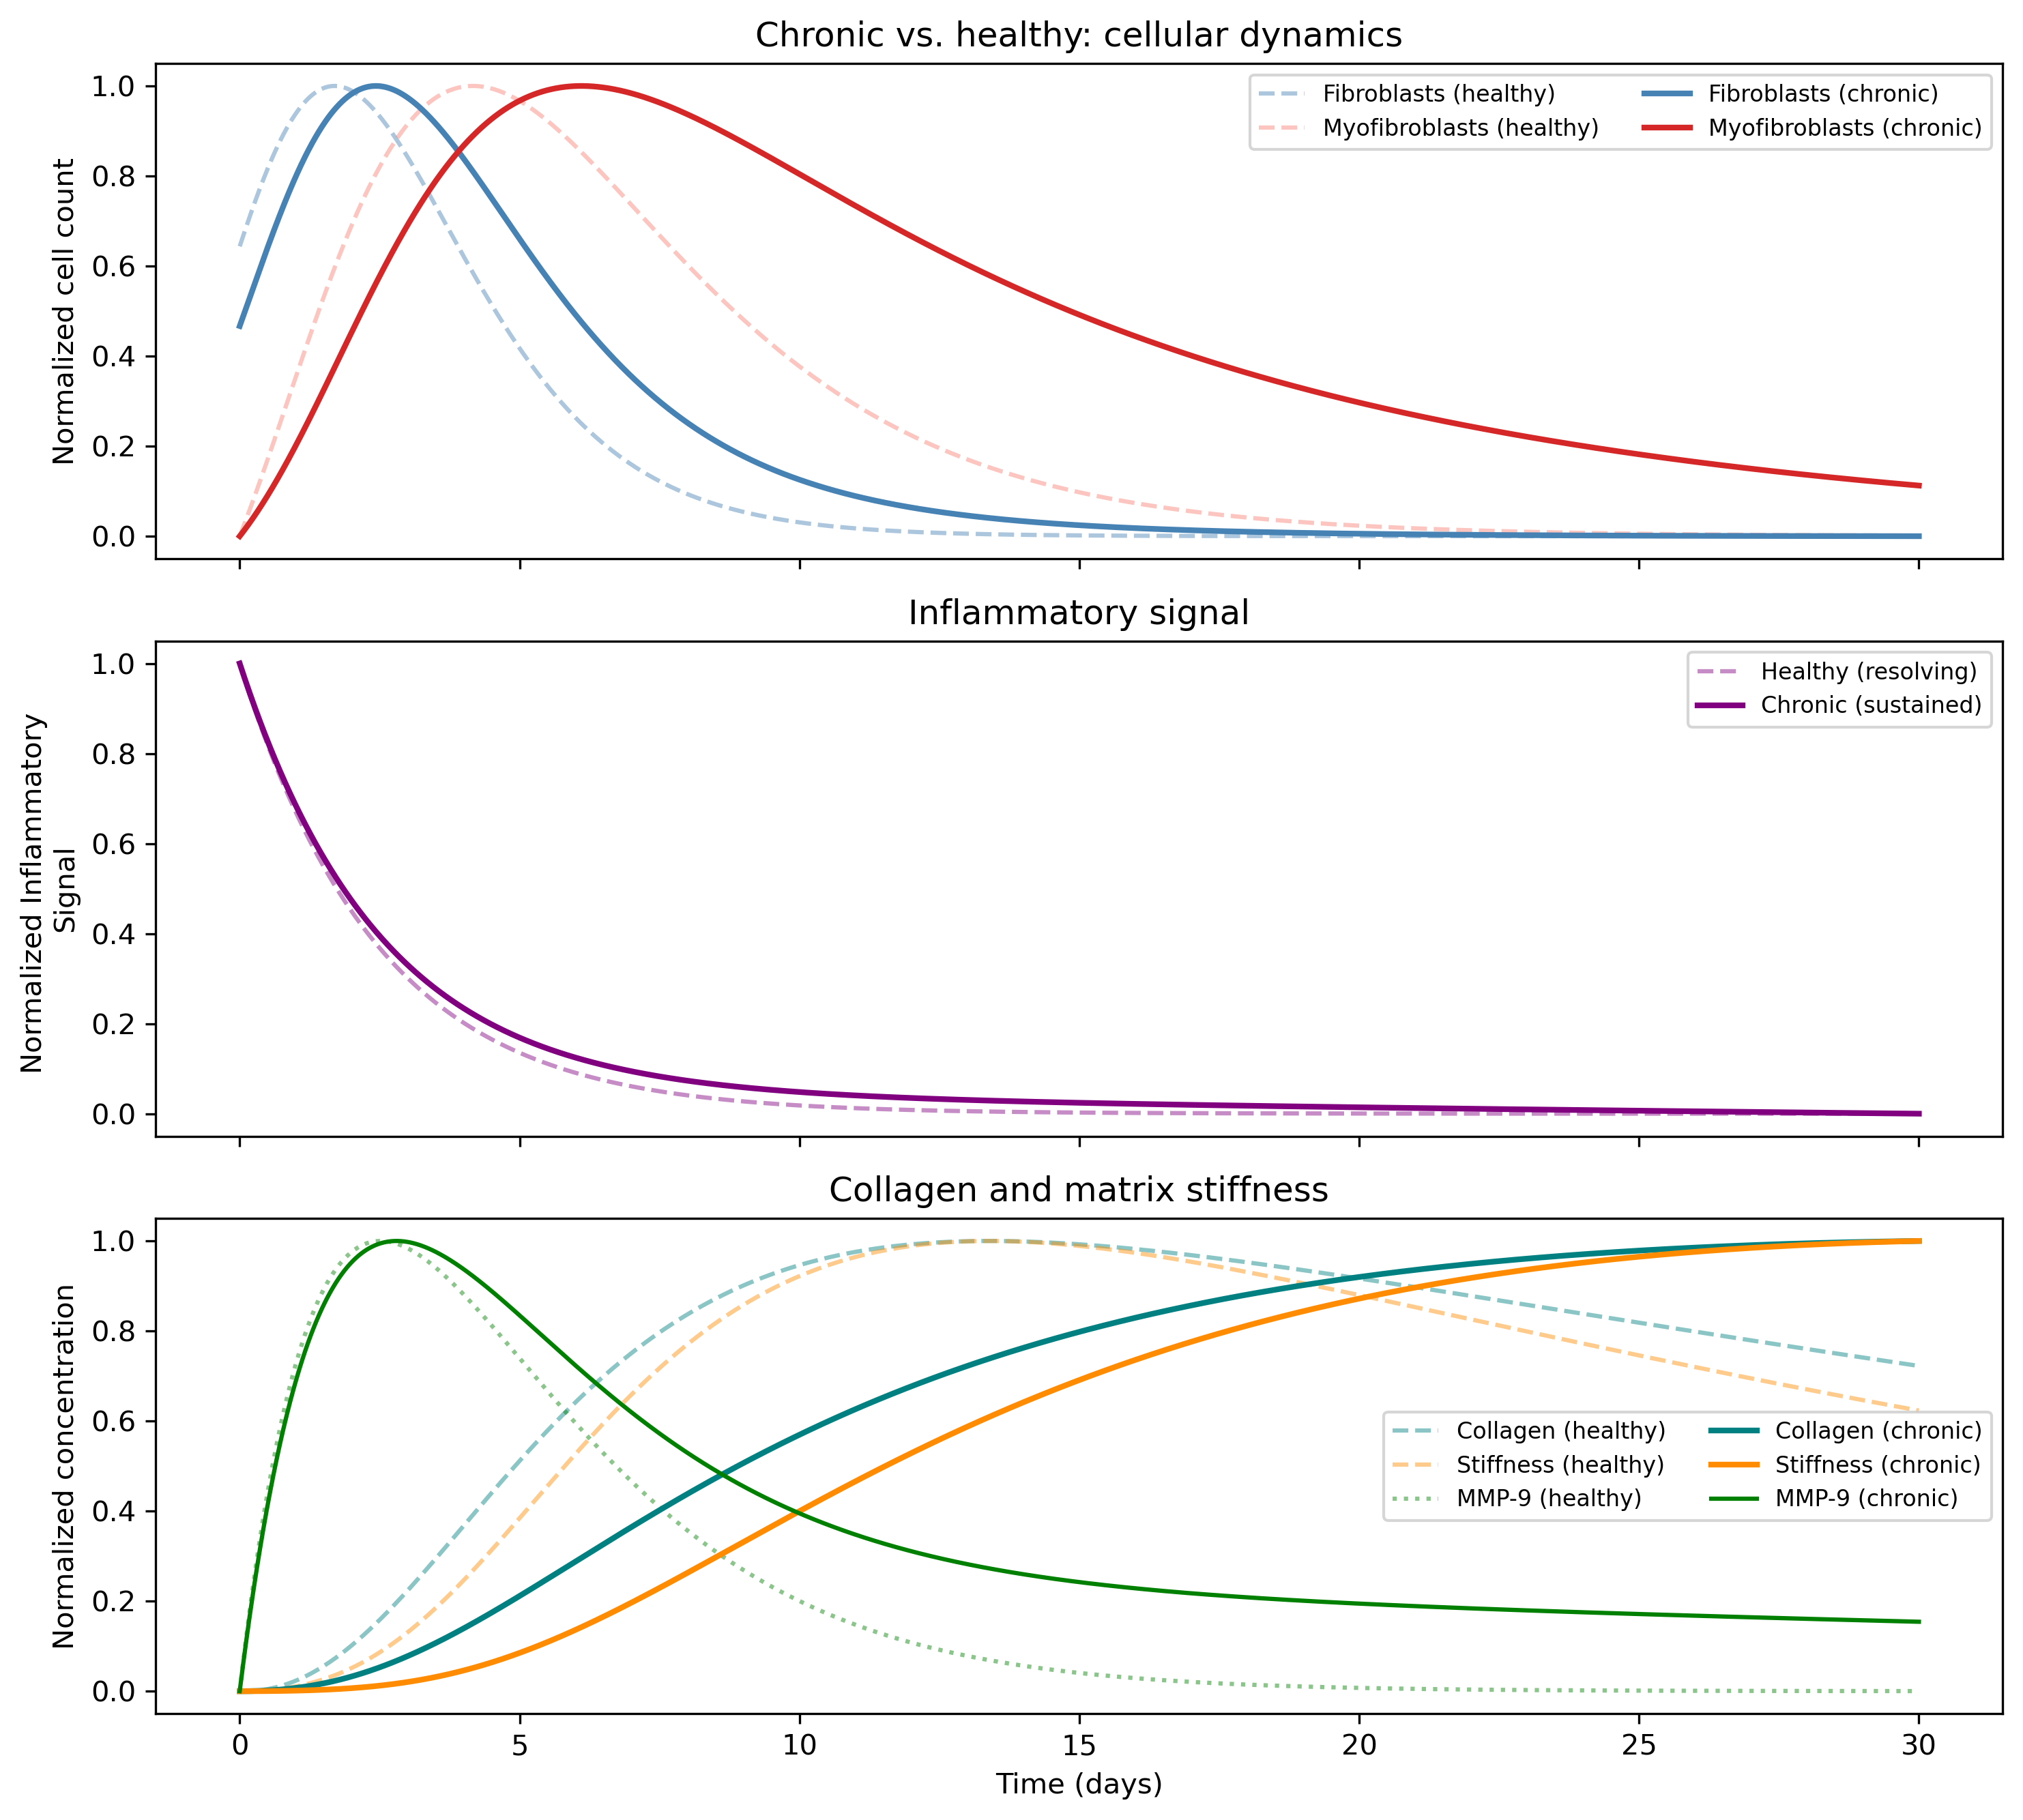
\includegraphics[width=\linewidth]{figures/fig_chronic_inflammation.png}
    \caption{Chronic inflammatory state (solid lines) overlaid on the healthy baseline (dashed lines) responses post myocardial infarction. Top: normalized fibroblast and myofibroblast cell count response. Middle: normalized IL-1$\beta$ concentration. Bottom: normalized collagen, stiffness, and MMP-9 concentration.}
    \label{fig:chronic-inflammation}
\end{figure*}

Figure \ref{fig:chronic-inflammation} compares the baseline (`healthy') healing response with a chronic inflammatory scenario. In the baseline case the inflammatory signal decays after the initial infarction and the inflammatory signal gradually returns toward a no inflammatory state. Fibroblast and myofibroblast populations rise shortly after the inflammatory spike, collagen increases as scar tissue forms, and all variables slowly decline as the wound healing process resolves.

The chronic case behaves very differently. In this simulation a persistent low-amplitude inflammatory signal was added and several parameters were shifted to represent a more fibrotic microenvironment (stronger stiffness feedback, slower collagen degradation, and slower myofibroblast decay). Under these conditions fibroblast activation lasts much longer and myofibroblasts remain elevated through the end of the 30-day simulation. Collagen and stiffness continue increasing rather than stabilizing, which is consistent with progressive fibrotic remodeling.

One noticeable difference between the two cases is that matrix remodeling activity does not fully resolve in the chronic scenario. MMP-9 levels approach a nonzero steady state, suggesting that extracellular matrix turnover remains active rather than shutting down after scar formation. This persistent remodeling behavior is often associated with pathological fibrosis in experimental studies~\citep{jin2011combining}.

\subsection{Sub-threshold vs.\ Supra-threshold Inflammatory Pulses}
\label{subsec:pulses}

\begin{figure*}
    \centering
    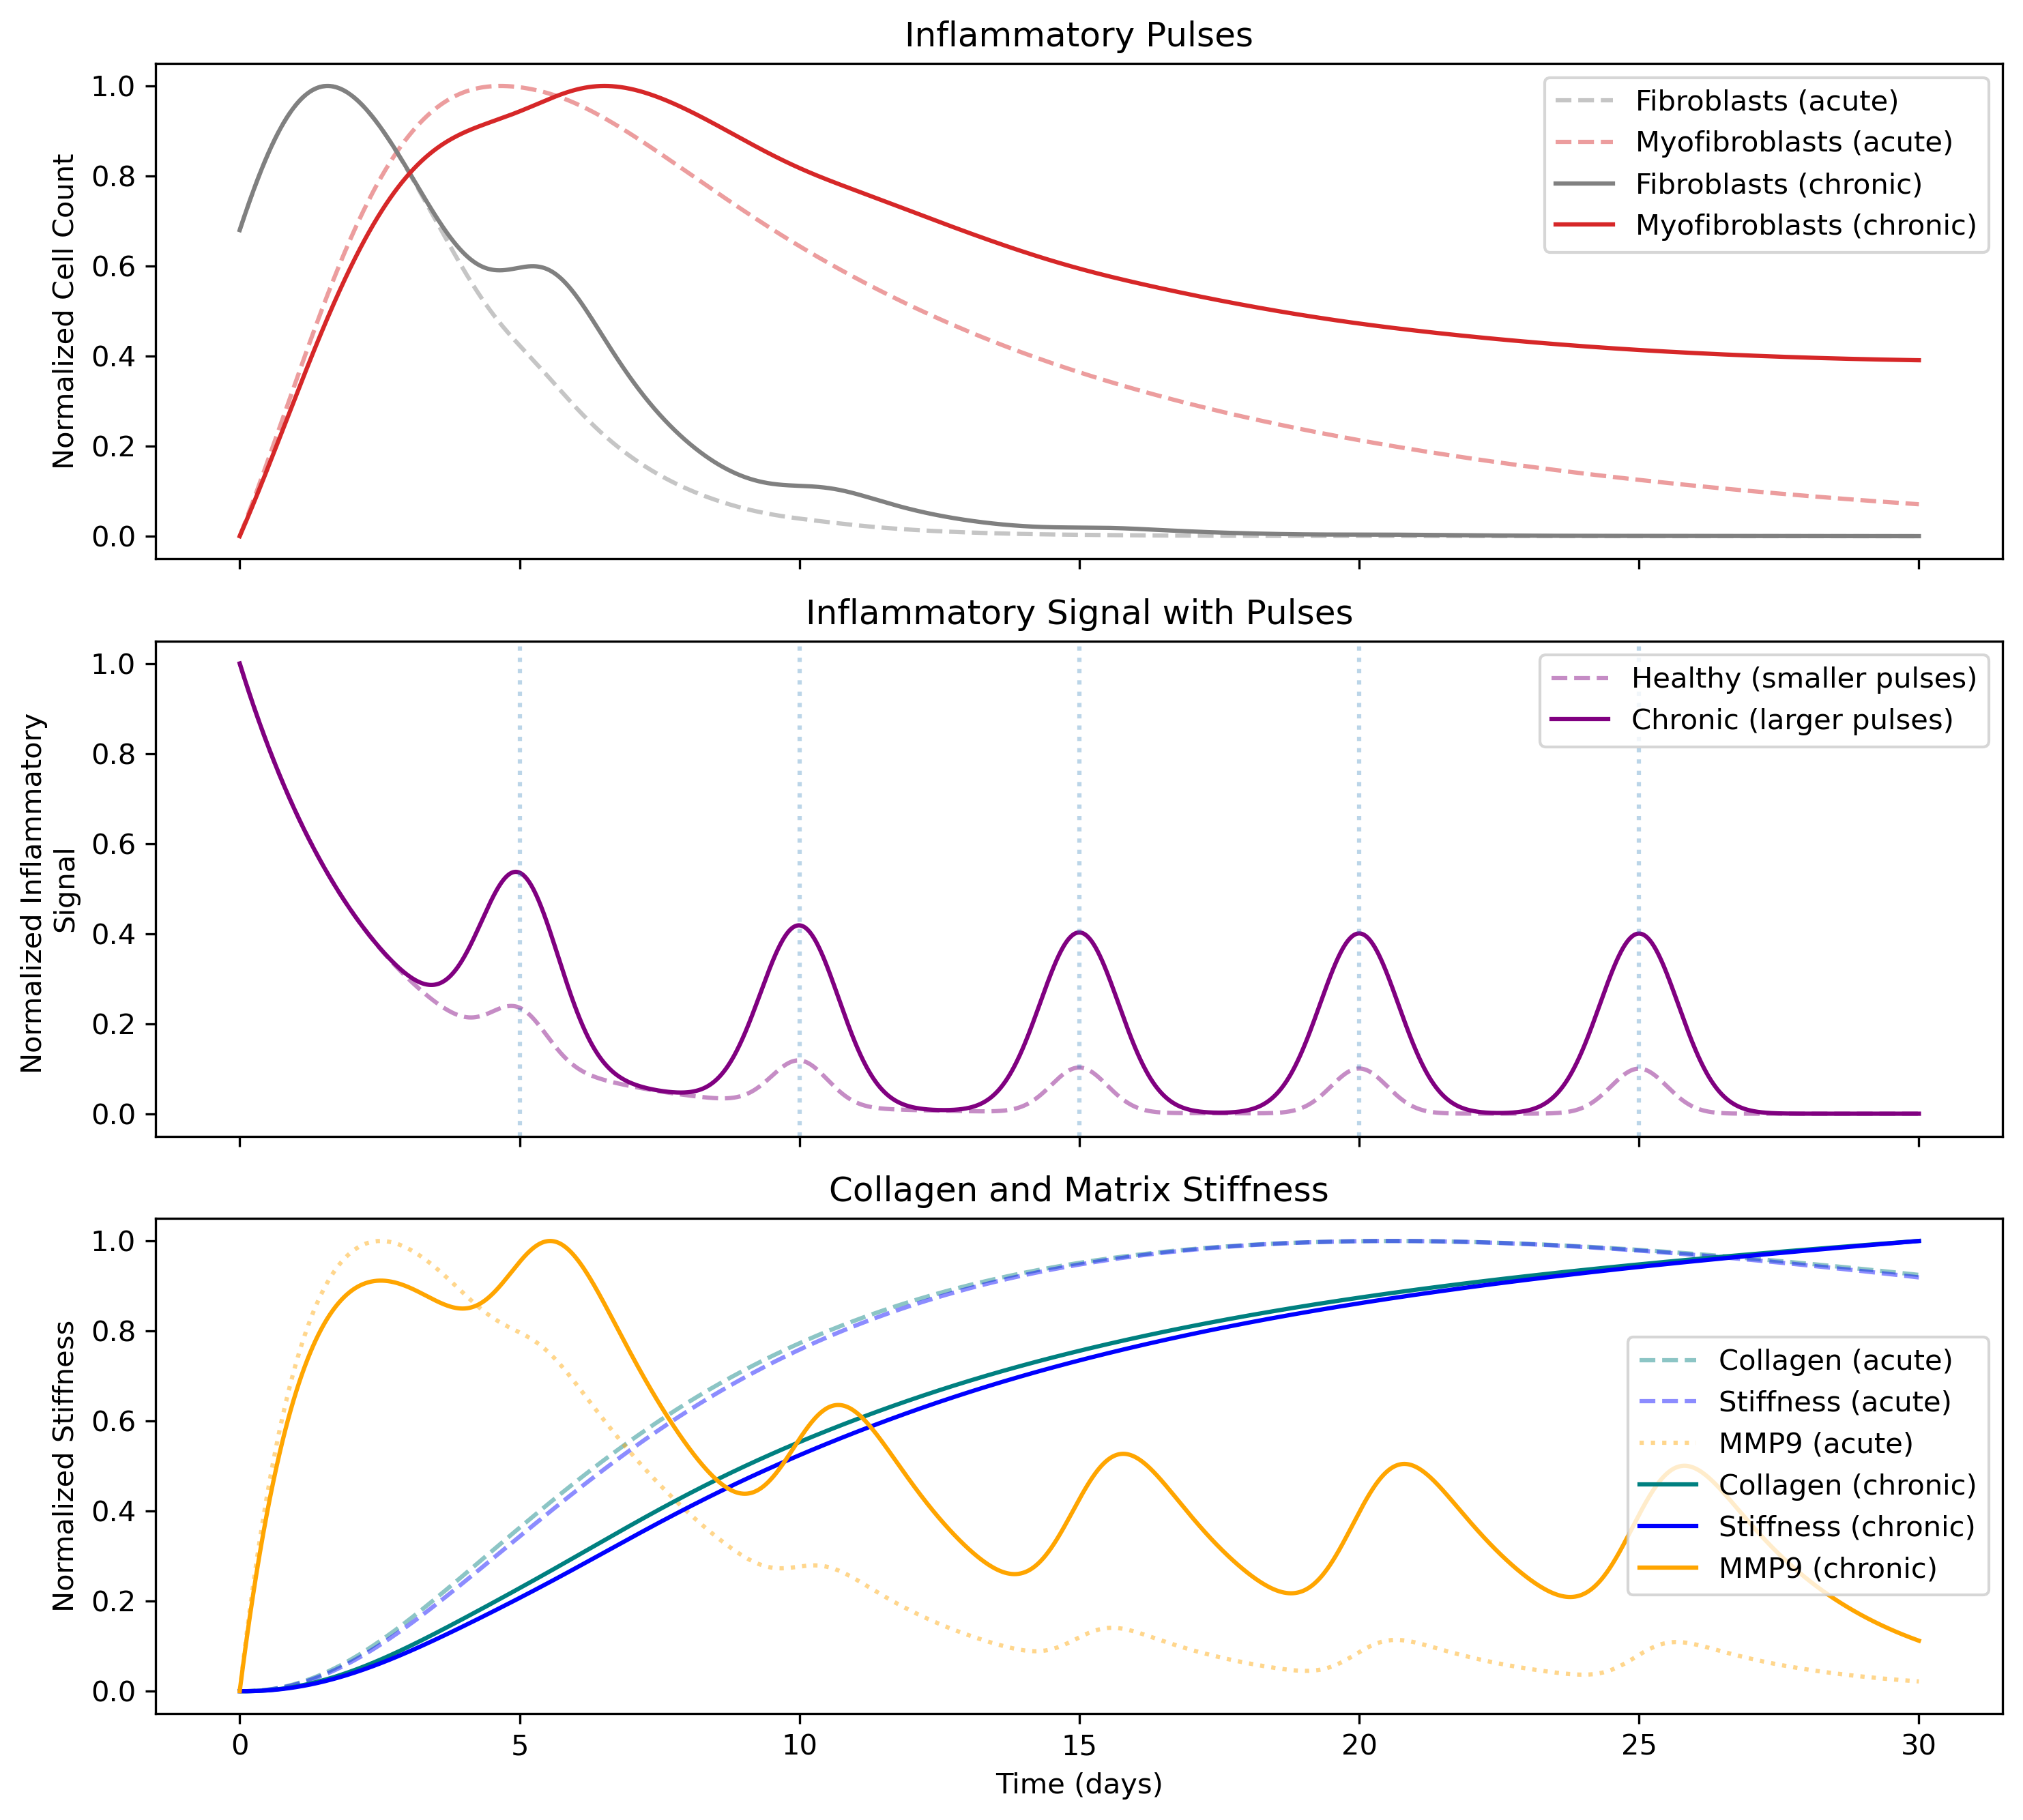
\includegraphics[width=\linewidth]{figures/fig_inflammation_compare_pulses.png}
    \caption{Response to five sub (dashed) and supra (solid)-threshold inflammatory pulses (amplitude $A = 0.1, 0.4$, width $w = 0.5, 2$~days respectively) at $t = 5, 10, 15, 20, 25$~days, superimposed on the initial MI spike. Top: normalized fibroblast and myofibroblast dynamics. Middle: normalized IL-1$\beta$ concentration. Bottom: normalized collagen, stiffness, and MMP-9 concentration.}
    \label{fig:small-inf-pulse}
\end{figure*}

To directly perturb the bistable nature of the model, we simulated two inflammatory pulse scenarios against the healthy baseline: five pulses of amplitude $A = 0.1$ and width $w = 0.5$~days (sub-threshold), and five pulses of amplitude $A = 0.4$ and width $w = 0.7$~days (supra-threshold), both applied at $t = 5, 10, 15, 20, 25$~days post-MI. Each individual pulse in the small case carries approximately one-tenth the inflammatory burden of the initial infarction spike, while each large pulse carries approximately two-fifths the infarction burden.

In the sub-threshold case (dashed lines of Figure~\ref{fig:small-inf-pulse}), the fibroblast and myofibroblast dynamics are qualitatively indistinguishable from the healthy baseline. This demonstrates that the model satisfies a key design criterion such that small repeated inflammatory insults do not irreversibly tip the system toward fibrosis.

In the supra-threshold case (solid lines of Figure~\ref{fig:small-inf-pulse}), the behavior is qualitatively different. Myofibroblasts remain chronically elevated and show no sign of returning to baseline by day 30, even as fibroblasts approach a steady state, indicating that the stiffness-driven $k_{SM} \cdot S/(S+K_S) \cdot M$ feedback term in Equation~\ref{eq:myofibroblasts} is sustaining myofibroblast activation independently of continued fibroblast input. Collagen and stiffness increase continuously through the end of the simulation window, consistent with the system having crossed into the high-stiffness stable fixed point of the bistable landscape. In a longer simulation this inflammatory signal would eventually resolve, but the collagen and stiffness would not, as the feedback loop is by this point self-sustaining.

The contrast between these two scenarios constitutes there exists a threshold of inflammatory input above which the feedback loop becomes self-reinforcing and the system commits irreversibly to a fibrotic state, and below which normal scar resolution proceeds.

\subsection{Sensitivity Analysis}
\label{subsec:sensitivity}

\begin{figure*}
    \centering
    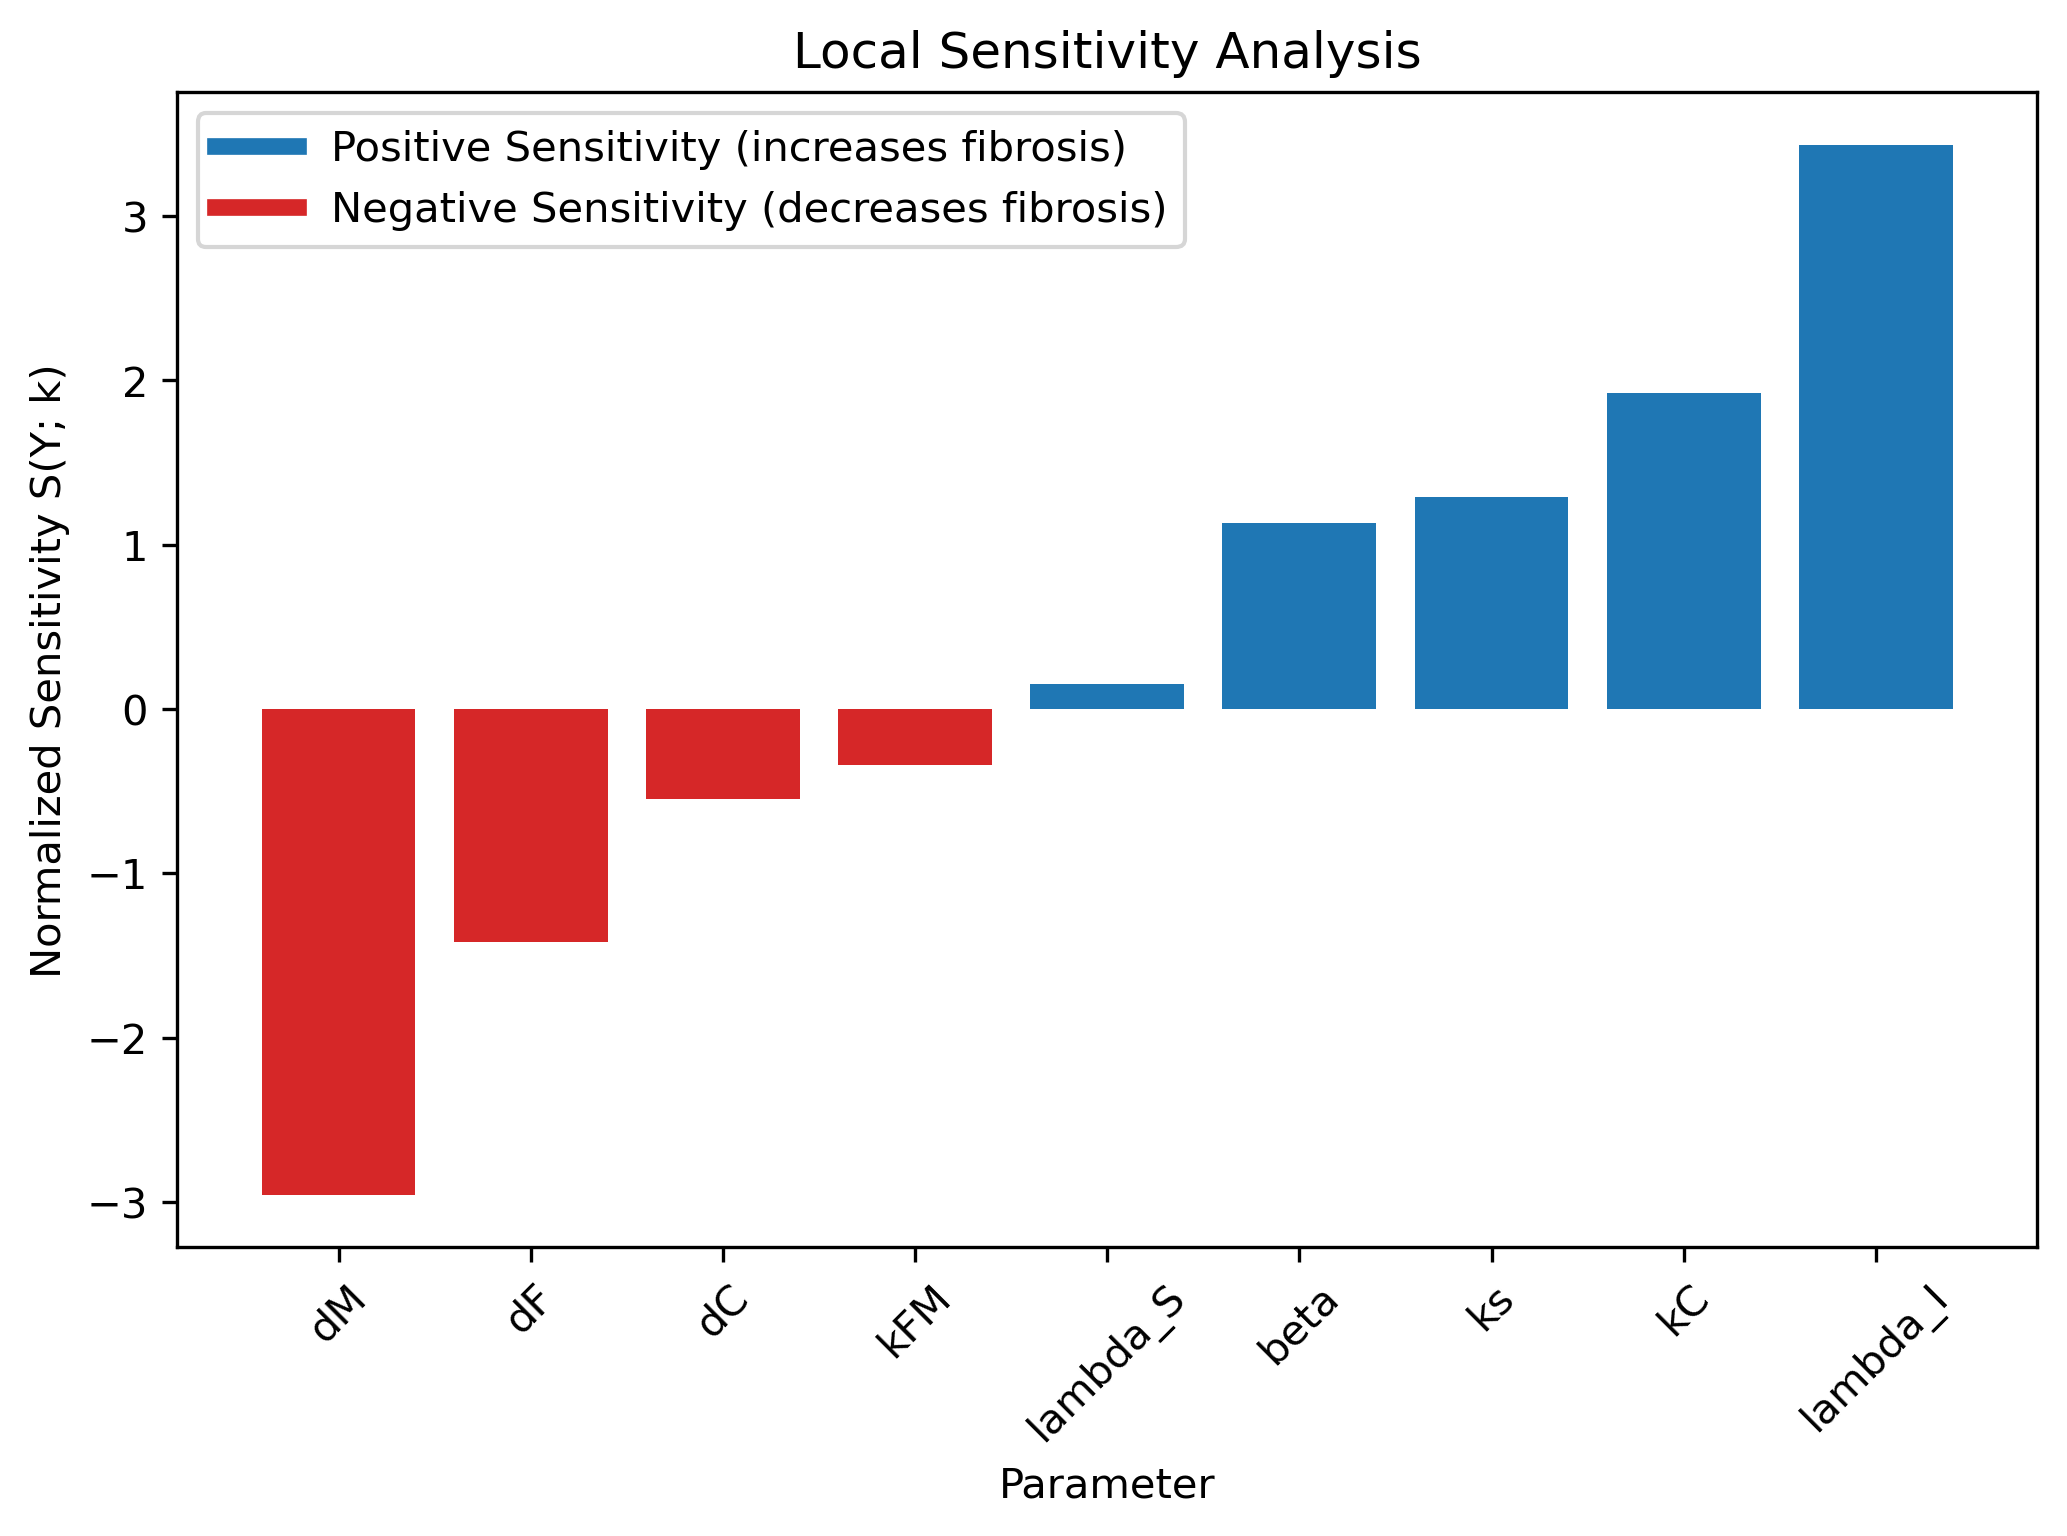
\includegraphics[width=\linewidth]{figures/fig_sensitivity_analysis.png}
    \caption{Local sensitivity analysis of steady-state collagen concentration $C(t=30)$ with respect to twelve model parameters, computed using the finite-difference formula in Equation~\ref{eq:sensitivity} with a 10\% symmetric perturbation. Blue bars indicate parameters whose increase raises steady-state collagen (pro-fibrotic); red bars indicate parameters whose increase reduces steady-state collagen (anti-fibrotic). Parameters with sensitivity indistinguishable from zero are omitted.}
    \label{fig:sensitivity}
\end{figure*}

A local sensitivity analysis was performed to determine which parameters most strongly influence steady-state collagen levels. Each parameter was perturbed by $\pm$5\% and the resulting change in final collagen concentration at day 30 was calculated using the normalized sensitivity coefficient defined in Equation~\ref{eq:sensitivity}.

The results are shown in Figure~\ref{fig:sensitivity}. Among the tested parameters, the inflammation driven fibroblast recruitment rate ($\lambda_I$) and the myofibroblast decay rate ($\delta_M$) have the largest effects on steady-state collagen accumulation. This is not surprising because these parameters directly control how quickly collagen is produced and how long the collagen-producing cells persist.

The collagen degradation rate ($\delta_C$) also shows a strong negative sensitivity, indicating that faster matrix turnover substantially reduces collagen accumulation. Parameters associated with myofibroblast collagen production rate ($k_C$) and stiffness-mediated recruitment ($\lambda_S$) have moderate positive sensitivities, reflecting their role in sustaining the feedback loop.

Overall, the sensitivity analysis highlights which mechanisms most strongly control the fibrotic outcome in the model. Processes that regulate myofibroblast persistence or collagen production appear to have the largest impact on final matrix accumulation.


\section{Conclusions}
\label{sec:conclusions}

This study developed a simplified mechanotransduction model to investigate how inflammation and extracellular matrix feedback can lead to either normal wound healing or persistent cardiac fibrosis after myocardial infarction. The model captures key features of post-infarction remodeling by linking inflammatory signaling, fibroblast activation, collagen deposition, and stiffness-mediated feedback. Simulation results demonstrate two distinct healing trajectories. In the baseline case, inflammation resolves over time and fibroblast activity gradually declines, leading to stabilization of collagen levels and matrix stiffness. In contrast, simulations with sustained inflammatory signaling or sufficiently strong inflammatory pulses produced prolonged myofibroblast activation and continued collagen accumulation, consistent with a chronic fibrotic remodeling response. These results support the idea that fibrosis can arise when inflammatory signals push the system past a critical threshold, after which feedback maintains collagen production even after inflammation subsides.

Sensitivity analysis further indicated that parameters governing collagen production and myofibroblast persistence have the strongest influence on long-term matrix accumulation. This suggests that biological processes controlling fibroblast activation and extracellular matrix turnover play a central role in determining fibrotic outcomes. Overall, the model reproduces several qualitative features observed in experimental studies of post-infarction remodeling, including the coupling between inflammation and fibrosis and the potential for threshold-driven fibrotic transitions. While the model is intentionally simplified and does not capture all cell types or signaling pathways involved in cardiac healing, it provides a useful framework for exploring how inflammatory perturbations and mechanical feedback interact to regulate fibrosis.

\bibliographystyle{vancouver}
\bibliography{references}

\appendix

\section{Work Summary}
\label{sec:work}

\subsection{Python Code}\label{sec:code}

All code and results are available on GitHub:
\href{https://github.com/caterer-z-t/CHEN_5150/tree/main/Midterm}{repository link}. 
This directory contains Jupyter notebooks (\texttt{.ipynb}) for the simulations, sensitivity analyses, and figures presented in this report. Figure~\ref{fig:model_schem} was created in \texttt{draw.io} and is present in the \texttt{./figures} directory. 

\subsection{Report Formatting}
\label{sec:tex}

This report was prepared using \LaTeX{} to align with the assignment requirement that the manuscript be ``formatted similarly to articles published in biological engineering journals''. The document uses the Sage Publications \textit{Journal of Tissue Engineering} \LaTeX{} template. For transparency, the complete source files for this report (including the \texttt{.tex}, \texttt{.cls}, \texttt{.bls}, and \texttt{.bib} files and compiled PDF, and all accompanying files) are available in the accompanying GitHub repository referenced in the above Section (in the \texttt{./paper} directory).

\subsection{Disclosure and Dissent}
\label{sec:disclosure}

Generative artificial intelligence tools were used to assist with this project. All generated content was reviewed, edited, and verified by the authors, who take full responsibility for the accuracy, integrity, and final content of this work. 

The authors wish to record a note of dissent regarding the administrative constraints surrounding this assignment. Due to limited flexibility in deadlines that overlapped with prior commitments, and notice of the full scope of project and expectations, completing this project required substantial adjustments to personal and professional schedules to meet the required timeline. Consequently, the work presented here was prepared with careful attention to the criteria outlined in the grading rubric and the instructions provided. To ensure that evaluation is commensurate with the stated rubric and assignment guidelines, the authors request that any evaluative comments be clearly linked to those criteria. Where concerns arise, we would appreciate clarification regarding the specific expectations involved and how they were intended to be inferred from the materials provided.

\end{document}